\chapter{Background}

% To have a better understanding of our approach, it's important to understand the basic concept and assumption that we used to develop the approach. 

\section{\ac{VHR} Aerial Imagery}

\begin{figure}[H]
    \centering
    \includegraphics[width=\textwidth]{Figures/arz_7_resolution_compare.png}
    \caption[Resolution Comparison]{Comparison between different resolutions. From left to right, where (a) has 300 dpi, (b) has 200 dpi and (c) has 100 dpi. With the number of dpi decrease, it harder to capture the boundary of the edge detail of sidewalk.}
    \label{fig:vhr_compare}
\end{figure}

\ac{VHR} stands for Very High Resolution, it's advantageous for buildings extraction, road detection or image segmentation\cite{FREIRE20141, 10.1007/BFb0015525, 10.1007/978-3-642-15567-3_16}. These aerial imageries contain more information and detail due to the higher resolution, which gives us the ability to process more complex analysis on the imagery with same size. \figref{fig:vhr_compare} demonstrates the difference between the same area with different resolution. From (a) to (c), the resolution changes from 300 \ac{dpi} to 100 \ac{dpi}, with higher resolution, it's easier to find the precious boundaries of an object or identify it. For building extraction, with the technique to combine 2-D edge information, photometric and chromatic attributes with 3-D information \cite{10.1007/BFb0015525}, higher resolution provide more information when dealing with complex houses or extract complex suburban roofs. For thin ribbon-features such as sidewalks in our approach, when to visualize an overland map, without high resolution, the imagery can be distracting, and the output may effect by tiny discrepancies between digitized  pathways\cite{10.1007/978-3-642-15567-3_16}. 

\section{\ac{OSM}}
\begin{figure}[H]
    \centering
    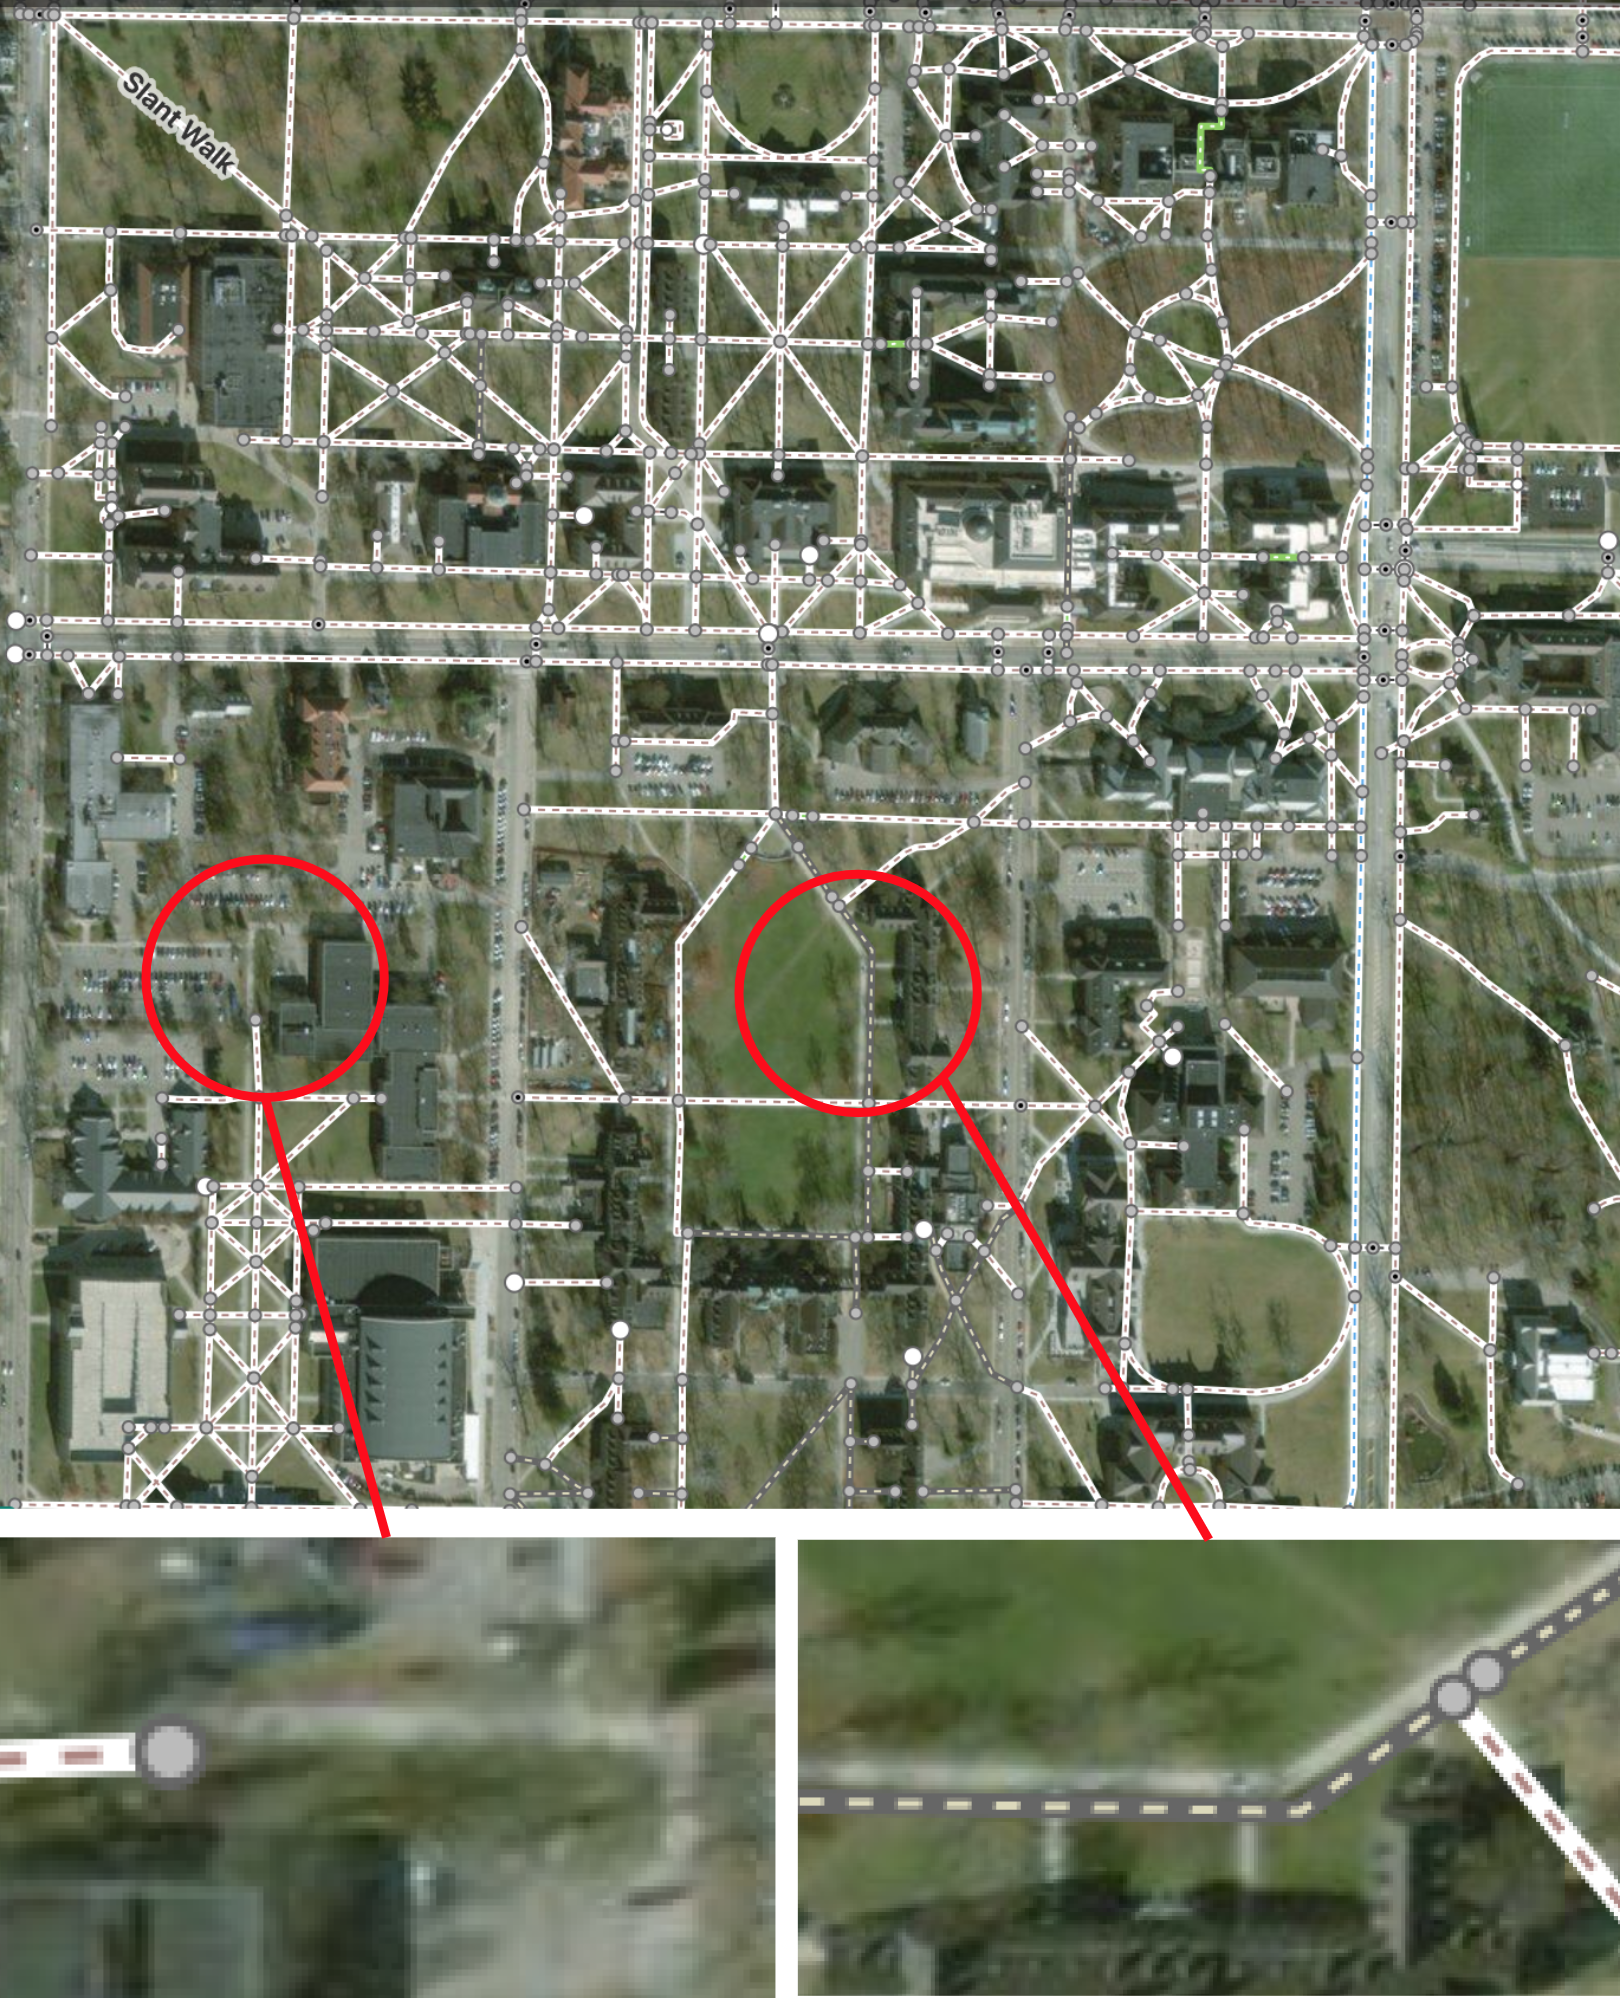
\includegraphics[width=\textwidth]{Figures/oxford_path_data_osm.png}
    \caption[\ac{OSM} Walking Path]{A demonstration on extract the path data from \ac{OSM}. This is a time-saving process by avoiding hand mark all the sidewalk location with given data set. The figure shows in the Oxford area in Ohio, US.}
    \cite{OpenStreetMap}
    \label{fig:osm_oxford_path}
\end{figure}
\ac{OSM} stands for Open Street Map, which founded by Steve Coast in 2004 \cite{lasPiñas, OpenStreetMap}. \ac{OSM} is a collaborative project that allows users to generate a free editable map of the world \cite{4653466}. Rather than the map itself, \ac{OSM} generate the data with map information that across most of the world as primary output. It also allows users to develop the map data with portable satellite navigation devices. With all these convenience features, \ac{OSM} is helpful for map analysis and feature segmentation \cite{10.1007/11744078_9}. \figref{fig:osm_oxford_path} shows that \ac{OSM} supports features like footpaths, roads, buildings, and others, with the ability to extract the \ac{GIS} data for any individual feature. It's a time-saving process when dealing with large data set, by given the ability to locate the \ac{GIS} data for each feature that we need to analyze. It may lead to the issue of dealing with missing or invalid data when we rely on the data set for auto-detection, or mismatch data with imagery when structures changes along time.

\section{\ac{CRF}}
\ac{CRF} stands for Conditional Random Field, which is a class of statistical modeling method that often applied in pattern recognition and machine learning \cite{MAL-013}. As a type of discriminative undirected probabilistic graphical model, \ac{CRF} is commonly used for segmenting, labeling or parsing of sequential data, such as in computer vision, structure segmentation and object recognition \cite{RuizSarmiento2015UPGMppA, 1315232, lafferty2001conditional}. For road segmentation, several approaches are able to locate the precise boundaries by treating it as a \ac{CRF} problem \cite{ActiveContou09, Achanta:149300}. 


\section{\ac{GMM}}

\ac{GMM} stands for Gaussian Mixture Model \cite{sridharan2014gaussian}.It is a probabilistic model for representing normally distributed subpopulations within an overall population. \ac{GMM} often can be performed when the data points are mixtures of a Gaussian distribution. It can be used in common computer vision tasks such as background and foreground subtraction \cite{1333992}. For road segmentation, we can treat the problem as subtract foreground (road feature) from the complex background (non-road feature). \figref{fig:gmm_sample_1} demonstrate the comparison between foreground and background \ac{GMM} on sample walking path show in grayscale. For foreground subtraction, which shown in row 1 and row 3, we treat sidewalk texture as foreground and apply the \ac{GMM} algorithm to subtract it from the background (non-sidewalk texture). Background subtraction are shown in row 2 and row 4, we did the opposite and treat non-sidewalk part as foreground. 

\begin{figure}[H]
    \centering
    \includegraphics[width=0.8\textwidth]{Figures/gmm_sample_1.png}
    \caption[\ac{GMM} Background Subtraction]{A demonstration of apply \ac{GMM} algorithm on sample inputs, show with gray scale. From top to bottom, row 1 shows foreground \ac{GMM} on sample path, row 2 show background \ac{GMM} on the same sample path as row 1. Same with row 3 and 4, with different sample path. For foreground \ac{GMM}, lighter color represent more likely to be sidewalk and darker color represent more likely to be non-sidewalk. Background \ac{GMM} shows as the opposite.}
    \label{fig:gmm_sample_1}
\end{figure}


\section{\ac{DP}}

\begin{figure}[H]
    \centering
    \includegraphics[width=\textwidth]{Figures/QVSdv.png}
    \caption[Demonstration on Fibonacci Sequence]{Representing the calculation of Fibonacci Sequence ($7^{th}$) with binary tree. Without applying dynamic programming, it need's certain exponential rate to calculate $n^{th}$ Fibonacci number. With the increase of $n$, the number of calculation increase significantly.}
    % \cite{stack_overflow}
    \label{fig:fbs}
\end{figure}

\ac{DP} stands for Dynamic Programming. It's both a mathematical optimization method and a computer programming method \cite{bertsekas2005dynamic}. In 1950s \ac{DP} was invented by Richard Bellman\cite{bellman2013dynamic}. The main concept of \ac{DP} is to simplify a complicated problem by breaking it down into simpler sub-problems in a recursive manner \cite{howard1966dynamic}. In computer science, if a problem can break into serial sub-problems and each sub-problem can be recursively solved by finding it's optimal solution, then we know that \ac{DP} are applicable. 

Dynamic Programming has a variety of applications since it can significantly reduce the run-time \cite{bertsekas1995neuro}. We use Fibonacci Sequence to demonstrate the \ac{DP} process\cite{horadam1961generalized}. Figure \ref{fig:fbs} shows that to calculate the $n^{th}$ Fibonacci number, it require a certain exponential rate of calculation to finish the process. The time complexity can be reduced since it's re-calculating the previous Fibonacci number repeatedly. By applying \ac{DP} algorithm, we can save the previous calculated Fibonacci number and reused it when needed. Figure \ref{fig:fbs_dp} indicate the same process after applying dynamic programming, we marked unnecessary steps in red X. By trade in linear space to save previous calculation, we can reduce the wrong time from exponential to linear.

\begin{figure}
    \centering
    \includegraphics[width=\textwidth]{Figures/QVSdv_DP.png}
    \caption[Demonstration on Fibonacci Sequence with \ac{DP}]{Representing the calculation of Fibonacci Sequence ($7^{th}$) with binary tree. With dynamic programming, after saving previous calculation, it's only require linear time steps to calculate $n^{th}$ Fibonacci number. We marked unnecessary steps in red X to show it's can be skipped.
    }
    % \cite{stack_overflow}
    \label{fig:fbs_dp}
\end{figure}

% \section{Street Network Extraction}
% boss paper, 2018 cvpr, they don't gurant to find the center of road.

